% Observed results only. The root report supplies inference definitions,
% fixed-source null checks, the preamble, and the running figure counter.
\clearpage\section*{2016 extraction: separate the window and template changes}

The 2016 scan compares three choices on the same spectrum: the inherited Gaussian in its original window; that same Gaussian in the MC-centered $[-3.5,+3.5]u$ fit and training-exclusion interval; and the neighboring MC template in that interval. The intermediate choice isolates the window change before changing the signal shape.

\begin{center}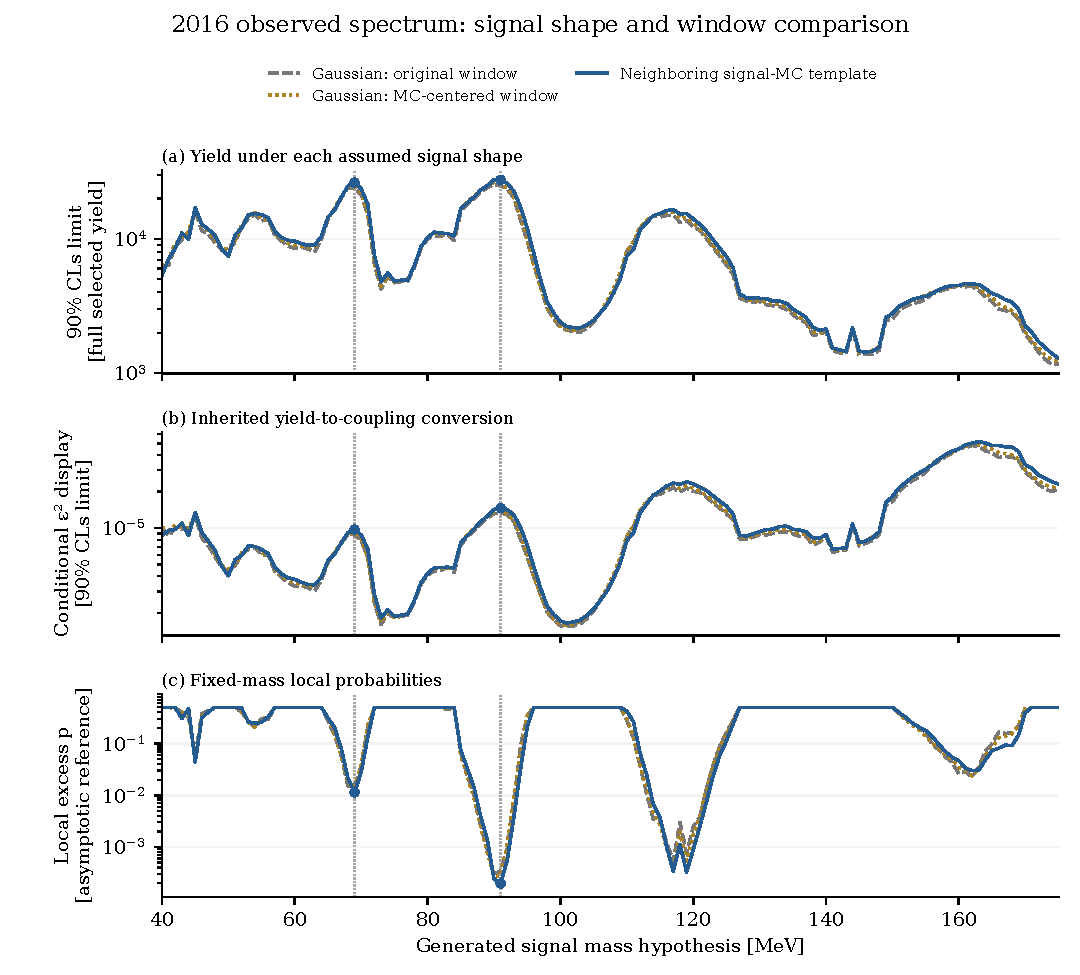
\includegraphics[width=\linewidth,height=4.8in,keepaspectratio]{../figures/extraction_2016_scan.pdf}\end{center}
{\small\refstepcounter{figure}\textbf{Figure \thefigure. How to read the figure.} Gray: the inherited Gaussian centered at the generated mass, with the original $\pm2.25\sigma_{\rm ref}$ interval. Gold: the same Gaussian with the MC-centered fit and exclusion interval. Blue: the neighboring MC template in that interval. Top: observed 90\% profile-CLs limits on each assumed shape's full selected yield. Middle: the inherited conditional conversion to the $\epsilon^2$ display. Bottom: fixed-mass asymptotic excess probabilities. Blue points identify the two regions shown next. The Gaussian and MC curves describe different signal-shape assumptions; their limits are not interchangeable calibrations of an MC-shaped signal.}\par\medskip

Across the 136 tested masses from 40 to 175 MeV, changing only the window changes the upper limit by a median $+3.6\%$, with a range of $-1.3\%$ to $+10.4\%$. Replacing the Gaussian with MC at that fixed window adds a median $+3.2\%$, with a range of $-14.8\%$ to $+20.6\%$. These summarize the observed scan, not an uncertainty distribution.

The smallest local asymptotic probability moves from $3.08\times10^{-4}$ at 90 MeV for the original Gaussian to $2.75\times10^{-4}$ at 91 MeV for the window control, then $1.96\times10^{-4}$ at 91 MeV for MC. These are local references selected from a mass scan. The fixed-source null checks are discussed separately; none of these minima is a global discovery probability.

\clearpage\section*{2016: the strongest selected region, at 91 MeV}

The MC fit returns a signed full selected yield of $20{,}201\pm5{,}699$ events. Its core is at 90.731 MeV with width 3.492 MeV. The actual fitted bins cover 78.50--103.00 MeV and contain 99.27\% of the selected template probability. The signal yield still refers to the complete template.

\begin{center}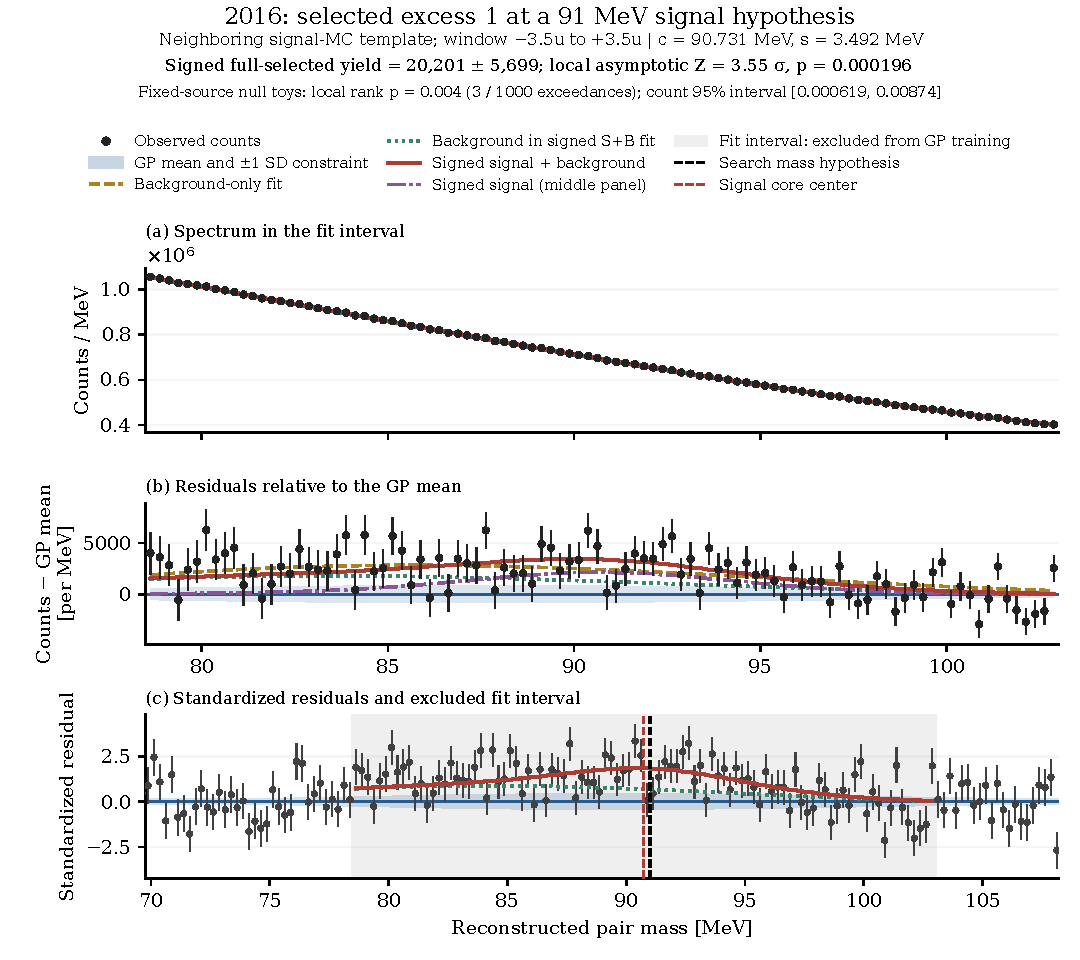
\includegraphics[width=\linewidth,height=5.7in,keepaspectratio]{../figures/extraction_2016_excess_1.pdf}\end{center}
{\small\refstepcounter{figure}\textbf{Figure \thefigure. How to read the figure.} Black points are observed counts with square-root-count errors. Blue is the GP sideband prediction with its marginal one-standard-deviation constraint band. Gold is the profiled background-only fit; green is the background component of the signed signal-plus-background fit; red is its total. The middle panel subtracts the GP mean and shows the signed signal in purple. The bottom panel standardizes residuals by $\sqrt{b_{\rm GP}+V_{{\rm GP},ii}}$ and shades the excluded fit interval. The black and red vertical lines mark the generated hypothesis and MC core. Profiled curves appear only in the fitted bins. The blue band is a background constraint, and the correlated residuals are not independent significance measurements.}\par\medskip

At this same 91 MeV hypothesis, the upper yield limit is 25,048 events for the original Gaussian, 26,031 for the Gaussian window control, and 27,505 for MC. The corresponding local asymptotic significances are 3.40, 3.46 and 3.55. The null-toy annotation provides a separate conditional reference: three of 1,000 toys exceed the observed MC statistic, giving the add-one rank $4/1001$. Its interpretation and finite-sample interval are treated in the null-check discussion.

\clearpage\section*{2016: the second distinct region, at 69 MeV}

The second displayed region, at 69 MeV, is the strongest remaining local maximum with fitted bins disjoint from the 91 MeV region. The 117 and 119 MeV maxima have smaller local probabilities but overlap that fitted interval; they remain visible in the full scan.

\begin{center}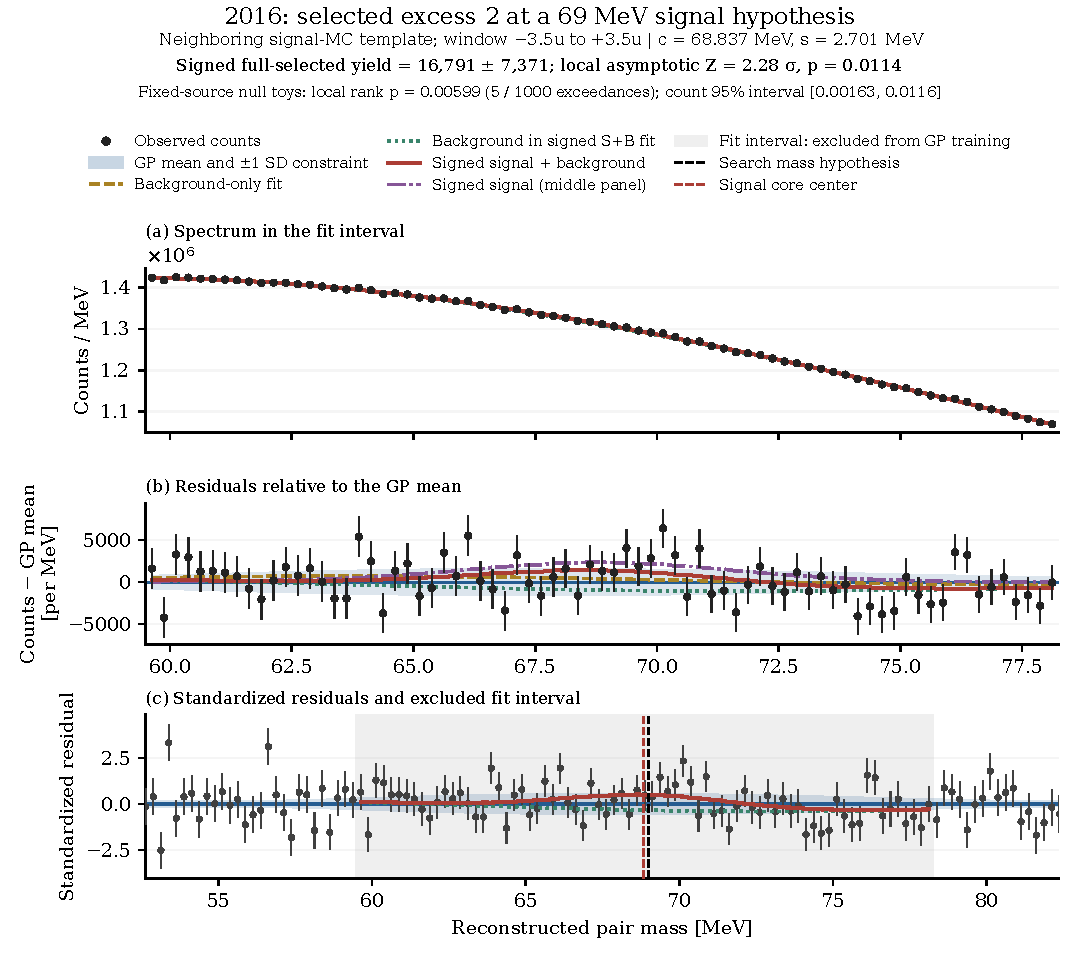
\includegraphics[width=\linewidth,height=5.05in,keepaspectratio]{../figures/extraction_2016_excess_2.pdf}\end{center}
{\small\refstepcounter{figure}\textbf{Figure \thefigure. How to read the figure.} The three panels and curves use the same definitions as the preceding fit: observed spectrum, residuals relative to the GP prediction, and standardized residuals including neighboring sidebands. The actual fit and training-exclusion interval is 59.50--78.25 MeV. The template core is at 68.837 MeV with width 2.701 MeV; 99.29\% of its selected probability lies in the fitted bins. Its quoted yield retains full selected normalization. The two displayed fit intervals are disjoint, but their GP sidebands overlap, so they are not independent tests.}\par\medskip

The fitted MC yield is $16{,}791\pm7{,}371$ events, with a local asymptotic probability of 0.0114. At 69 MeV, the upper yield limit changes from 23,750 events for the original Gaussian to 24,800 for the Gaussian window control and 26,285 for MC. The MC conditional coupling display is $\epsilon^2_{90}=9.74\times10^{-6}$.

Five of the 1,000 fixed-source null toys exceed the observed statistic, giving the add-one rank $6/1001$. This rank and its interval describe the specified null source at this mass. Choosing the region using the observed scan is not included in that probability. The report's null-check discussion explains the distinction between these ranks and the dense asymptotic curves.

\clearpage\section*{Combine the campaigns with three signal prescriptions}

The combined comparison starts from the established Gaussian analysis, replaces 2021 with neighboring MC, then also replaces 2016 with neighboring MC. The 2015 Gaussian is retained throughout. The all-Gaussian reference \emph{already uses the established logarithmic core shift for 2021}.

\begin{center}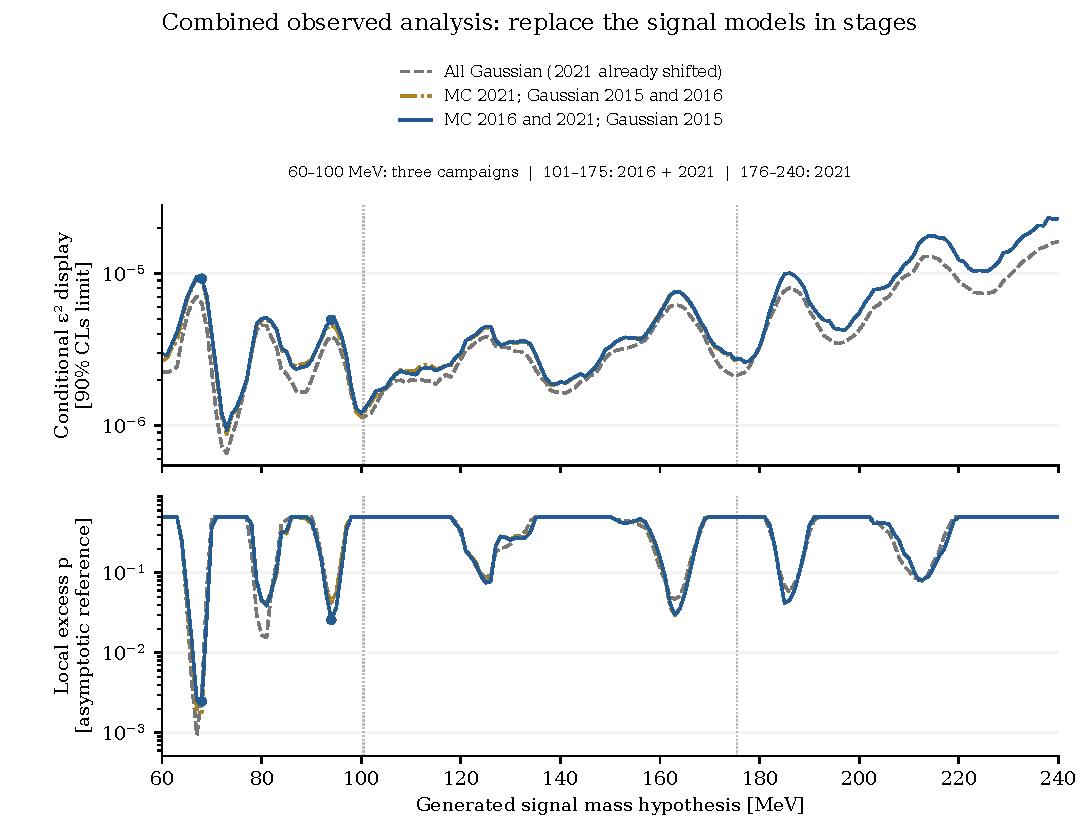
\includegraphics[width=\linewidth,height=4.2in,keepaspectratio]{../figures/extraction_combined_comparison.pdf}\end{center}
{\small\refstepcounter{figure}\textbf{Figure \thefigure. How to read the figure.} Top: conditional observed 90\% profile-CLs limits in the inherited $\epsilon^2$ display. Bottom: local asymptotic excess probabilities. The two MC choices use $[-4,+3]u$ for 2021, and the final choice also uses $[-3.5,+3.5]u$ for 2016. Fit and GP-exclusion intervals change together. All curves use the same campaign support: 2015, 2016 and 2021 at 60--100 MeV; 2016 and 2021 at 101--175 MeV; and 2021 alone at 176--240 MeV. Vertical dotted lines mark these transitions. The two MC curves coincide above 175 MeV. Blue points mark the selected combined regions.}\par\medskip

\begin{center}\small\begin{tabular}{lrrr}\toprule
Combined signal prescription & Minimum at [MeV] & Local $p_0$ & Local $Z$\\\midrule
All Gaussian; 2021 shifted & 67 & $9.33\times10^{-4}$ & 3.11\\
2021 MC; 2015/2016 Gaussian & 68 & $1.81\times10^{-3}$ & 2.91\\
2016/2021 MC; 2015 Gaussian & 68 & $2.48\times10^{-3}$ & 2.81\\
\bottomrule\end{tabular}\end{center}

Thus the strongest combined local feature moves by 1 MeV and becomes less significant under the MC prescriptions. At the common 68 MeV hypothesis, the three upper-limit displays are $(6.35,\,9.05,\,9.26)\times10^{-6}$, respectively. The second selected combined region is at 94 MeV, with final-model $p_0=0.0257$ and $\epsilon^2_{90}=4.97\times10^{-6}$. These observed-selected local results retain the inference qualifications given in the method and null-check sections.

\clearpage\section*{Which campaign shapes the combined result?}

The common-coupling fit uses each campaign's own observations, background constraint and signal template. Individual excesses therefore need not reinforce one another at the same generated mass. The individual curves below help explain the combined result without treating their probabilities as quantities to multiply.

\begin{center}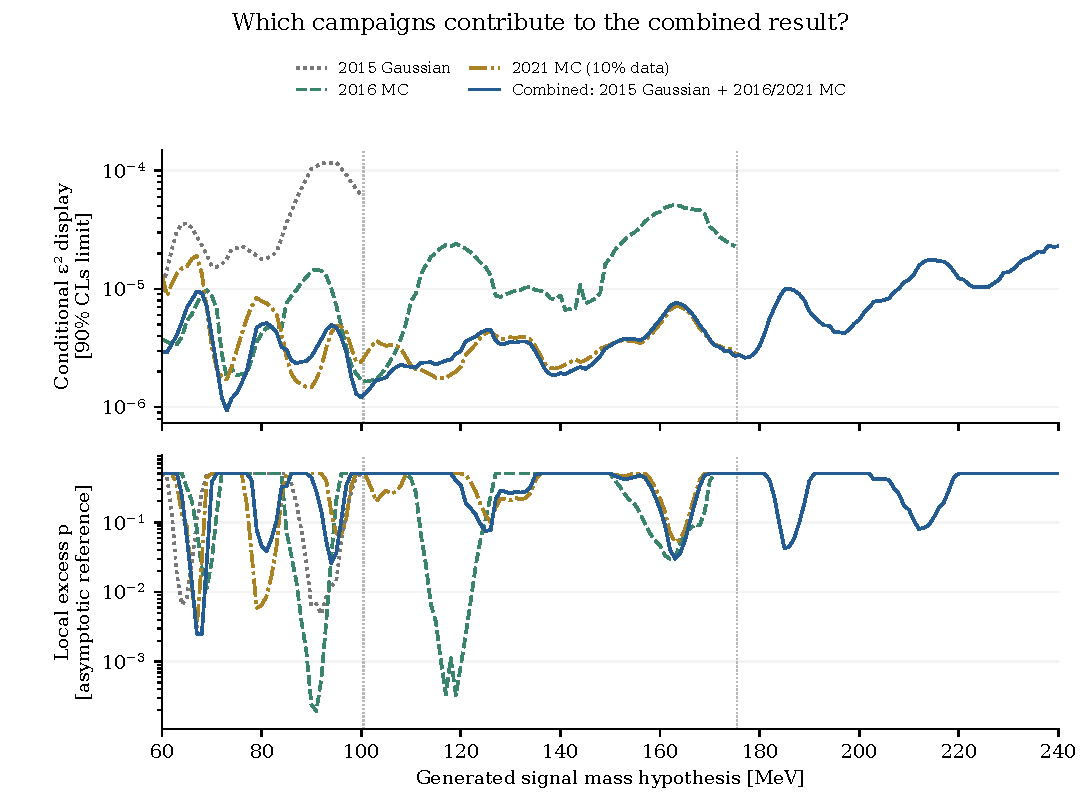
\includegraphics[width=\linewidth,height=5.15in,keepaspectratio]{../figures/extraction_campaign_contributions.pdf}\end{center}
{\small\refstepcounter{figure}\textbf{Figure \thefigure. How to read the figure.} Gray: the retained 2015 Gaussian. Green: the shifted 2016 MC template. Gold: the shifted 2021 MC template using the 10\% observed spectrum. Blue: their common-coupling profile combination, with separate GP constraints. Top: each conditional upper-limit display; bottom: each local asymptotic excess probability. The individual curves stop at their prescribed domain boundaries. Above 175 MeV, the combined curve is the 2021 curve. An observed combined upper limit need not be below every individual observed limit because the common signal parameter must describe all included datasets.}\par\medskip

At 91 MeV, the signed likelihood roots are $+2.47$ for the 2015 Gaussian, $+3.55$ for 2016 MC, and $-1.58$ for 2021 MC. The combined root is only $+0.59$, corresponding to local $p_0=0.277$. The strongest 2016 feature consequently does not become the strongest combined feature. A deficit in one campaign is relevant to the joint likelihood even though its one-sided excess probability is displayed as 0.5.

At 68 MeV, all three signed roots are positive: $+0.64$, $+2.03$ and $+1.90$, respectively. Their common-coupling fit gives the final model's largest combined excess statistic, with local $Z=2.81$. These comparisons describe compatibility with one common signal strength; they do not independently qualify the inherited conversion or supply a global mass-search calibration.

\clearpage\section*{How much do the combined upper limits change?}

The ratio view separates the large effect of replacing the 2021 Gaussian from the additional effect of updating 2016. Every ratio compares limits at the same generated mass, with the same included campaigns and coupling conversion.

\begin{center}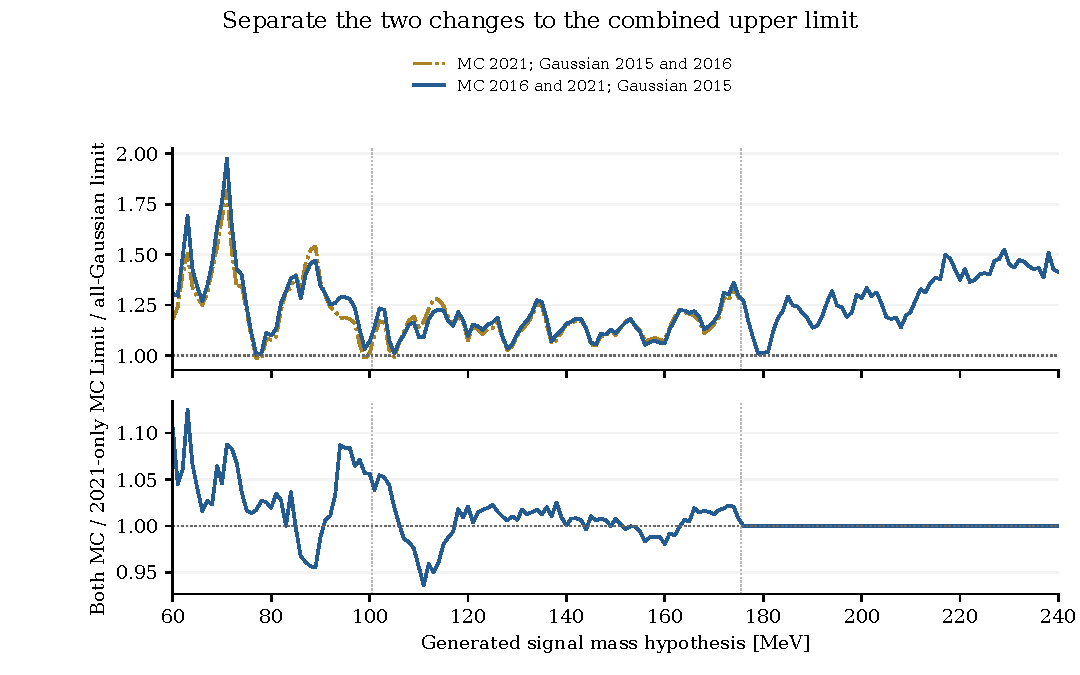
\includegraphics[width=\linewidth,height=4.25in,keepaspectratio]{../figures/extraction_combined_ratios.pdf}\end{center}
{\small\refstepcounter{figure}\textbf{Figure \thefigure. How to read the figure.} Top: each MC-based combined upper limit divided by the all-Gaussian combined limit. Bottom: the final model divided by the model that changes only 2021. One means no change; a value below one is a smaller conditional upper limit. The lower ratio is exactly one above 175 MeV because 2016 no longer contributes. These changes include both the assumed signal shape and its fit/training interval. They are not efficiency estimates or uncertainty bands.}\par\medskip

Across all 181 combined hypotheses from 60 to 240 MeV, replacing only 2021 changes the upper limit by a median $+19.5\%$, with a range from $-2.3\%$ to $+81.7\%$. Replacing both 2016 and 2021 changes it by a median $+21.8\%$ relative to the all-Gaussian reference, with a range from $+0.3\%$ to $+97.6\%$. The largest ratios occur at 71 MeV. These are descriptive summaries of the scanned observed limits; they are not repeated-experiment averages.

To isolate the added 2016 change, restrict attention to 60--175 MeV, where 2016 participates. Relative to the 2021-only MC result, adding 2016 MC changes the limit by a median $+1.3\%$, with a range from $-6.4\%$ at 111 MeV to $+12.5\%$ at 63 MeV. The change can have either sign because the signal shape and GP sidebands interact with the observed fluctuations.

\textbf{What the comparison establishes.} The final prescription has a defined shifted MC shape and exclusion interval for each of 2016 and 2021, while preserving the 2015 Gaussian. Its observed upper limits are generally higher than those from the inherited Gaussian comparison. A smaller local probability or a smaller limit would not, by itself, establish a better-calibrated procedure. The conditional conversion, the asymptotic limit construction and the finite null checks remain separate qualifications of the inference.
